\documentclass[conference]{llncs}
\usepackage{amssymb}
\usepackage{amsmath}
\usepackage{url}
\usepackage{hyperref}
\usepackage{amsopn}
\usepackage{listings}
\usepackage{graphicx}
\usepackage{etoolbox}
\usepackage{booktabs}
\usepackage{multirow}
\usepackage[noend]{algpseudocode}
\usepackage[font=footnotesize]{subfig}

\usepackage{tablefootnote}
\usepackage{bigstrut}

\usepackage{geometry}
\geometry{
  a4paper,         % or letterpaper
  textwidth=15cm,  % llncs has 12.2cm
  textheight=24cm, % llncs has 19.3cm
  hratio=1:1,      % horizontally centered
  vratio=2:3,      % not vertically centered
}

\newcommand{\union}{\cup}
\newcommand{\intersects}{\cap}
\newcommand{\refdefinition}[1]{Def.~\ref{#1}}
\newcommand{\reffigure}[1]{Fig.~\ref{#1}}
\newcommand{\refsection}[1]{Section.~\ref{#1}}
\newcommand{\reflemma}[1]{Lemma.~\ref{#1}}
\newcommand{\refexample}[1]{Example.~\ref{#1}}
\newcommand{\reftable}[1]{Table.~\ref{#1}}
\newcommand{\reftheorem}[1]{Theorem.~\ref{#1}}
\newcommand{\refequation}[1]{Equation.~\ref{#1}}
\newcommand{\refappendix}[1]{Appendix}
\newcommand{\refcorollary}[1]{Corollary.~\ref{#1}}
\newcommand{\zap}[1]{ }


\title{Hardware-Aware In-Memory Data Processing Systems}
\author{Chen Luo}
\institute{}

\begin{document}
\maketitle

\section{Introduction}
Large-scale Big Data analytics is becoming more and more critical for today's business, and lots of efforts have been made to improve the performance of data processing systems.
On one hand, larger volume of data are being produced in a even faster rate.
On the other hand, the advancement of modern hardware provides further opportunities for performance improvement.
For example, in-memory data processing can significantly improve response time and throughput~\cite{in-memory2015}.
From the user's prospective, it would be ideal to simply upgrade the hardware configurations to speedup data processing systems. However, this is often challenging in practice.
As the recent work~\cite{challenge2015} shows, naively using advanced hardware would not necessarily bring significant performance gains for today's data management and processing systems.
Thus, this motivates the \emph{hardware-aware in-memory data processing system} to fully unleash the power of modern hardware capabilities.

Developing a general purpose hardware-aware data processing system is challenging.
Besides the requirements for traditional data processing systems, e.g., scalability and fault-tolerance, the proposed system should also address the following additional requirements/challenges:
\begin{enumerate}
\item Hardware-awareness: Modern hardware architectures, like graphics processing units (GPU), non-uniform memory access (NUMA) architecture, non-volatile memories (NVM) and remote direct memory access (RDMA) network, could provide significant performance improvement, but only when operated properly.
For example, NUMA architecture has non-uniform memory access rate (local memory vs. remote memory), which requires proper data placement/access strategies to achieve better performance.
Thus, as a basic requirement, the system must be aware of the characteristics of modern hardware architectures to make full use of their power.

\item One-size-fits-many: While a specific algorithm can be bound to certain hardware architecture, the system must not.
To be a general purpose data processing system, the proposed system should be able to work with different hardware configurations, i.e., one size fits many.
More specifically, the proposed system should be capable of identifying the hardware configurations of the underling cluster, and automatically choose the optimal (or near-optimal) plan to process the query.
One should also keep in mind that the cluster is usually heterogeneous in practice, which poses further challenge for the system.

\item Extensibility: Due to the technical advancements of hardware industries, hardware capabilities may change quickly, e.g., lower cost per bit for NVM, more CPU cores and even new architectures.
The handle such changes, the system requires novel architectural design to be extensible so that the newly emerged hardware can be easily integrated/plugged into the system.
\end{enumerate}

The remaining of the proposal is organized as follows. \refsection{sec:related-works} briefly reviews the related works.
\refsection{sec:research-plan} proposes the preliminary design of the system and discuss how the above requirements are addressed.
Finally, \refsection{sec:conclusion} concludes the proposal.

\section{Related Works}
\label{sec:related-works}
In this section, we briefly review the state-of-the-art works on hardware-aware data processing.

To embrace modern hardware architectures, many hardware-aware query processing algorithms have been proposed~\cite{scan-numa2015,processing-gpu2015,join2015}.
The work~\cite{scan-numa2015} considers concurrent scan on columnar-stores on NUMA architecture.
Claude et at.~\cite{join2015} studies the problem of in-memory joins using RDMA network.
Join et al.~\cite{processing-gpu2015} proposes a query processing technique on CPU-GPU architectures.
All these works confirm that proper use of modern hardware architecture could lead to significant performance improvement.
However, these works only satisfy the requirement 1, i.e., hardware-awareness, but fail to achieve the requirements 2 and 3 due to the fact that they are bound to certain hardware architecture.

Besides the hardware-aware data processing algorithms, a lot of efforts have been made to develop efficient in-memory data processing systems~\cite{m3r2012,spark2012,platform2011}
M3R~\cite{m3r2012} is an in-memory extension of MapReduce~\cite{mapreduce2008}, but mainly targets at short-running jobs on high mean-time-to-failure clusters.
Spark~\cite{spark2012} is a general-purpose in-memory data processing system, and provides a data abstraction called Resilient Data Set (RDD).
The work~\cite{platform2011} extends MapReduce to support in-memory efficient stream data processing.
These systems only partially address the requirements 1 and 2, mainly for their in-memory and concurrent processing.
However, many advanced hardware architectures, like NUMA and RDMA, are still unexploited yet, and it is unclear how to plug new hardware architectures effectively into these systems (requirement 3).

\section{Research Design}
\label{sec:research-plan}
As discussed in the previous section, to the best of our knowledge, none of the existing works addresses the three requirements simultaneously.
In this section, we present the architectural design of the proposed hardware-aware in-memory data processing system, and briefly discuss the requirements are addressed.

\subsection{Architectural Design}
The architectural design is shown in \reffigure{fig:architecture}. Due to space limitation, we mainly discuss the components pertaining to the proposed system, while leave out the common components, e.g., master/ worker architecture, distribute file system and the DAG computation model.


\begin{figure}[t]
\centering
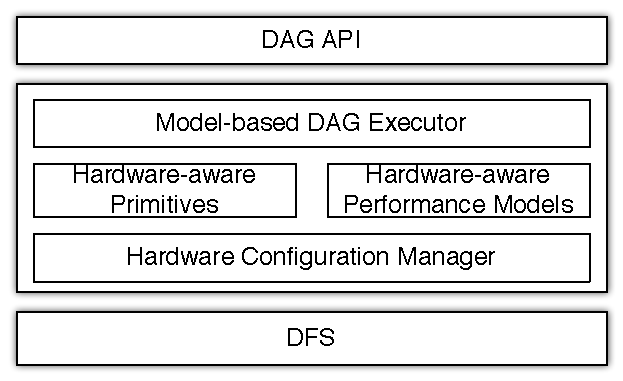
\includegraphics[width=0.45\linewidth]{architecture.pdf}
\caption{Architectural Design of the Proposed System}
\label{fig:architecture}
\end{figure}

\textbf{Hardware Configuration Manager}.
In order for the system to percept the underling cluster, the hardware configuration manager collects and manages the hardware information of all workers.
These information include but are limited to the memory sizes, number of CPU cores, memory/network read/write speed, the available hardware architectures (e.g., NUMA, RDMA, GPU, NVM) for each work.

\textbf{Hardware-aware Primitives.}
Each primitive can be viewed as a hardware-specific data processing operator, and the primitives together constitute the building blocks of the proposed system.
For example, there could be a hash join operator for normal network setting, and a join operator specially designed for RDMA network. 
These primitives include but are not limited to hardware-aware indexing, scan, join, group, aggregation etc.

\textbf{Hardware-aware Performance Models}.
For each hardware-aware primitive, there should be a corresponding performance model, which is used for the DAG executor to select the optimal execution plan.
These models could be parameterized with certain parameters, e.g., memory sizes, memory/network read/write speed and certain statistics of the dataset.
Note that these parameters may vary for different hardware architectures.

\textbf{Model-based DAG executor}.
With the performance models and the hardware configuration information of the clusters, the model-based DAG executor generates an optimal execution plan for the (logical) DAG task.
More specially, the executor formulates an optimization problem with the available hardware information, performance models and statistics of the dataset, and tries to find an optimal execution plan by solving the optimization problem.
The execution plan assigns certain workers to process certain input data with certain primitives, and shuffle the data when necessary with the chosen shuffling algorithm.
Moreover, the executor could also change the execution plan dynamically, and use approximate optimal plan to ensure timely response.

\zap{
With the architectural design, each query is processed as follows.
We assume each query is represented as a logical DAG task.
The DAG executor checks the hardware configuration of the cluster to determine the suitable data processing primitives, and formulate an optimization problem to determine the optimal execution plan.
With the execution plan, the executor assigns certain workers to process each DAG node with the chosen primitives, and shuffles data with the chosen shuffling algorithm when necessary.
}

\subsection{Addressing the Requirements}
We then briefly discuss how the proposed system addresses the three requirements.

The requirement 1 of hardware-awareness is naturally addressed by the hardware-aware primitives since each primitive corresponds to a specific hardware architecture to fully unleash its power.
For the requirement 2 of one-size-fits-many, the proposed system automatically collects the hardware information of the underling cluster, and choose the optimal execution plan based on the hardware configurations.
In other words, although the primitives are bound to certain hardware architecture, the system would try to find suitable primitives for the cluster so that the system is not bound to any specific hardware.

Finally, for the requirement 3 of extensibility, the proposed system could be easily adapted for the hardware changes.
Note that hardware could change in two ways, namely capacity changes or new hardware architectures.
For the first case, the changed capacity would be (ideally) automatically captured by the hardware configuration manager and the parameterized performance model.
While for new hardware architecture, the specific primitives should be developed and the corresponding performance models should be provided.
Moreover, the information of the new architecture should also be registered to the hardware configuration manager.
In practice, the maintenance would not cause too much effort, since the second case usually happens less frequently.


\section{Conclusion}
\label{sec:conclusion}
In this proposal, we discuss the requirements of hardware-aware data processing systems and review the current research status on this area.
We further propose an architectural design to address these requirements.
To make the system possible, a lot of efforts need to be made, including novel hardware-aware data processing primitives, performance models, and model-based DAG executor.
Moreover, extensive experiments should be performed to compare the proposed system with the existing systems, to study the maintenance effort of plugging new hardware and study the performance of the system in different and heterogeneous clusters.

\bibliographystyle{unsrt}
\bibliography{paper.bib}

\end{document}